\documentclass[11pt]{report}
\usepackage{eso-pic,graphicx}
\usepackage[export]{adjustbox}
\usepackage{url}
\usepackage[top=2cm, bottom=2cm, outer=2cm, inner=2cm]{geometry}
\begin{document}
%\AddToShipoutPictureBG*{
\includegraphics[width=\paperwidth,height=\paperheight]{images/bkgrnd}}
\begin{center}
\vspace*{2cm}
\textsf{\begin{Huge}
\textbf{ELP­718 ­ Telecom Software Laboratory \\
1st Semester, 2016-18 \\
Abhishek Mishra\\
18 Oct 2016, 5pm\\
Assignment-11}\\
\end{Huge}}
\vspace*{6cm}

\includegraphics[scale=0.12, center]{images/iitlogo}
\end{center}
\pagebreak
\tableofcontents
\vspace{5cm}
\pagebreak
\section{Introduction}
\vspace*{1cm}
This assignment aims to provide a better understanding of the following topics:\\

\begin{flushleft}
1. \textbf{Xilinx}\\
You may know Xilinx because we invented the FPGA. Or maybe you know us because we turned the semiconductor world upside down and created the fabless model. With over 3500 patents and more than 60 industry firsts, we continue to pioneer new programmable technology putting our customers first. Today Xilinx’s portfolio combines All Programmable devices in the categories of FPGAs, SoCs, and 3DICs, as well as All Programming models, including software-defined development environments. Our products are enabling smart, connected, and differentiated applications driven by 5G Wireless, Embedded Vision, Industrial IoT, and Cloud Computing.
\end{flushleft}

\begin{flushleft}
2. \textbf{VHDL}\\
VHDL (VHSIC Hardware Description Language) is a hardware description language used in electronic design automation to describe digital and mixed-signal systems such as field-programmable gate arrays and integrated circuits. VHDL can also be used as a general purpose parallel programming language.

\end{flushleft}
\newpage
\section{Problem Statement 1}
Model and simulate a 10 bit digital comparator with the following requirements:
Active low reset,Active low Chip select
Input- Two 10 bit words for comparison,a flip input bit/flag.
Output- 4 LEDs at the output for greater than,less than,equal and flipped mode status.

%	%\begin{figure}[h!]
%	%\centering
%	%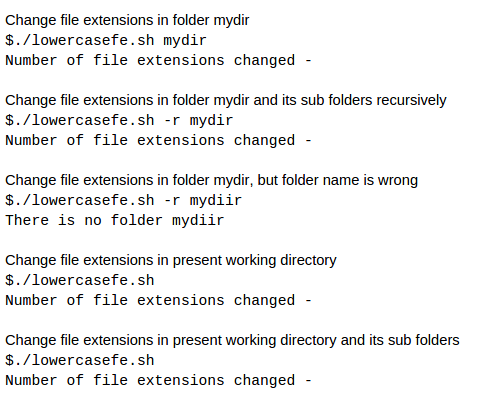
\includegraphics[scale=0.7]{images/Selection_003}	
%	%\end{figure}
\subsection{Assumptions}
The input bit streams do not change during testbench execution.
\subsection{Structure Chart and Implementation}
	\begin{figure}[h!]
	\centering
	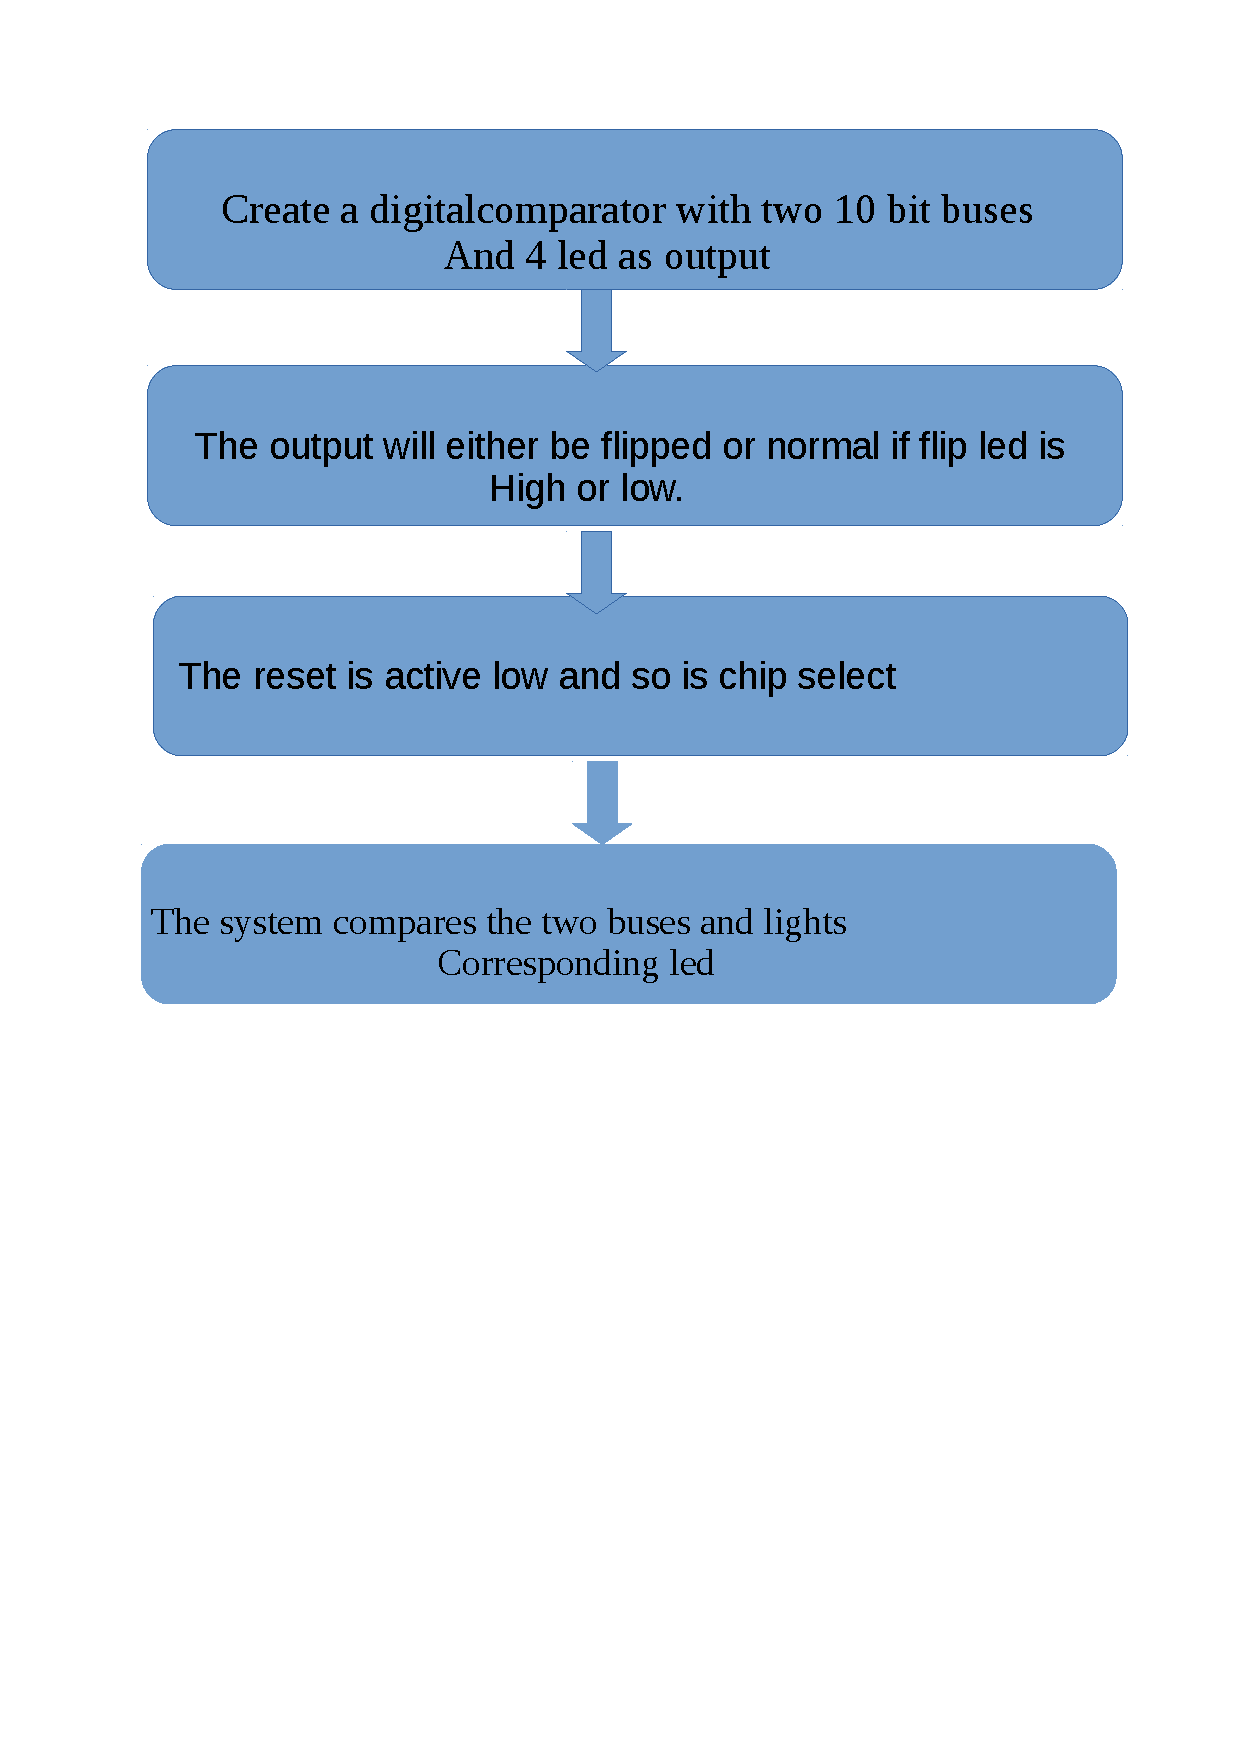
\includegraphics[scale=0.5]{images/shots11}
	\caption{Structure chart for problem 1}
	\end{figure}		
	\pagebreak
	\pagebreak
\subsection{Screenshots}
	\begin{figure}[h!]
	\centering
	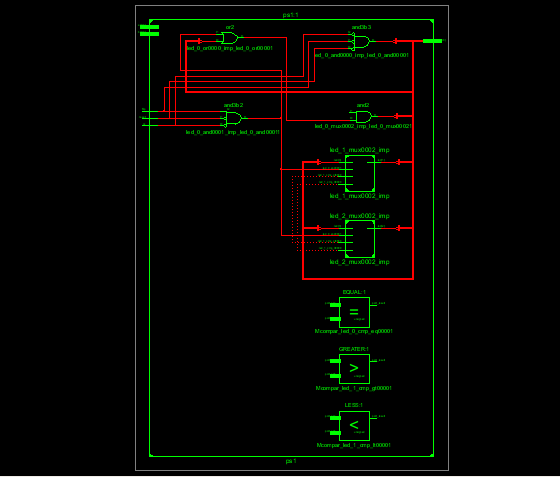
\includegraphics[scale=0.8, center]{images/screenshot11}
	\caption{Screenshot for problem statement 1}
	\end{figure}
	\begin{figure}[h!]
	\centering
	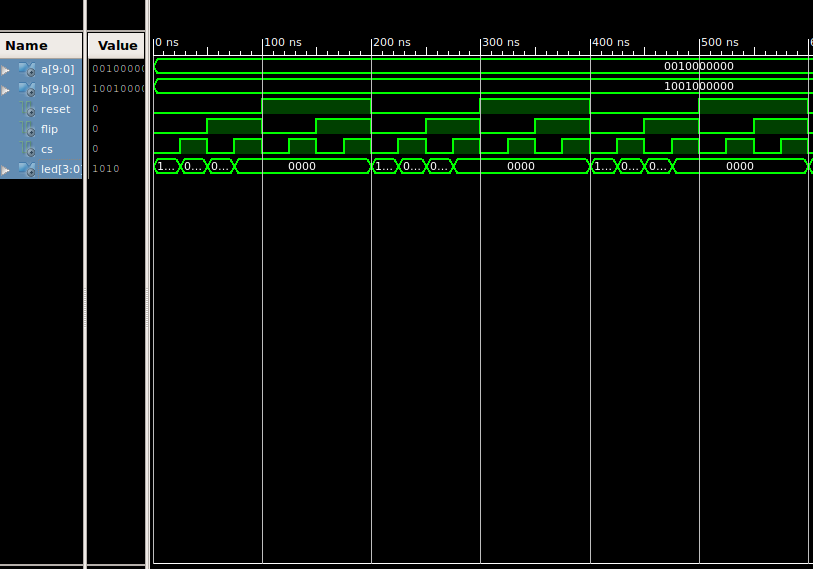
\includegraphics[scale=0.8, center]{images/screenshot12}
	\caption{Screenshot for problem statement 1}
	\end{figure}
	\pagebreak
%	%\iffalse
\section{Problem Statement 2}
Model a hardware for detecting a pattern of bits ‘11001’ in the input bit stream. The output LED must glow when the detection is successful.\\
Use Moore state machine for your design,simulate it in vhdl and generate the corresponding RTL for the same.Include an asynchronous reset input in the design for resetting to the initial state when the hardware is switched on.\\
\subsection{Assumptions}
Overlapping is possible.
\pagebreak
\subsection{Structure Chart}
	\begin{figure}[h!]
	\centering
	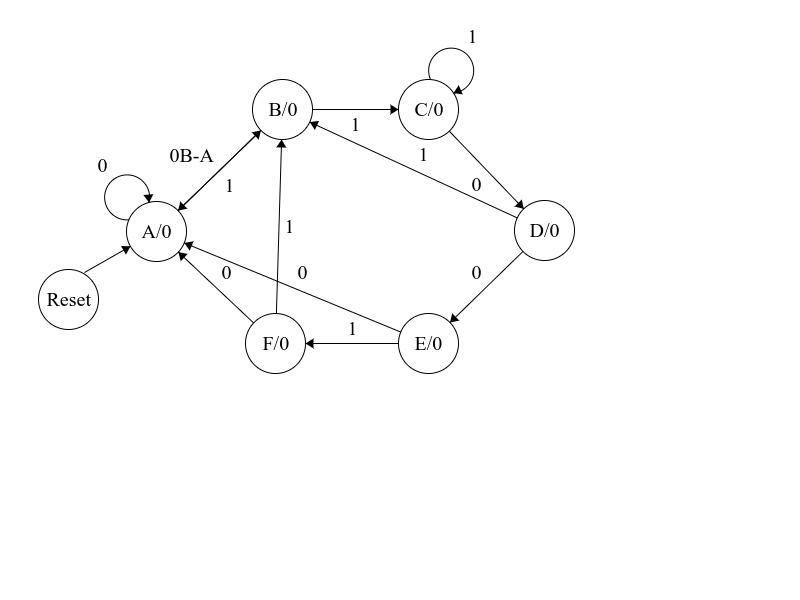
\includegraphics[scale=0.7]{images/shots21}
	\caption{Structure chart for problem 2 - moore implementation}	
	\end{figure}
	\pagebreak
	\begin{figure}[h!]
	\centering
	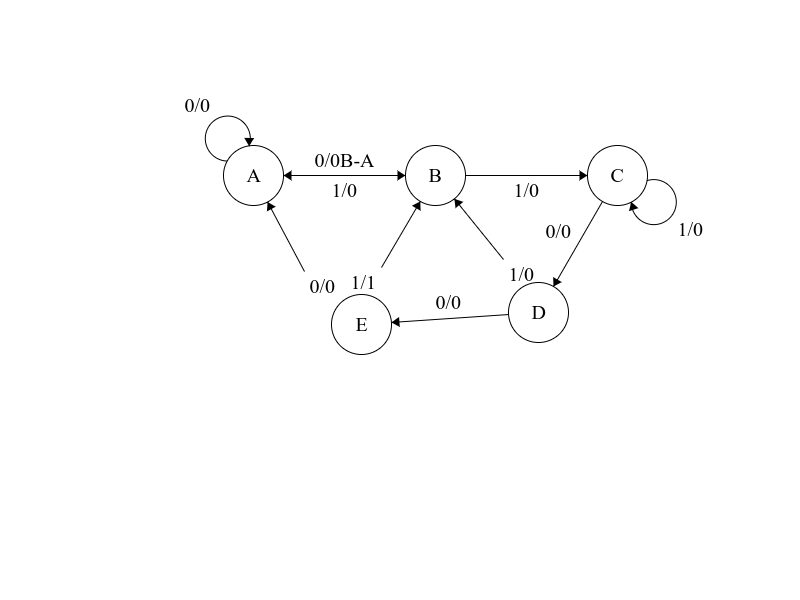
\includegraphics[scale=0.7]{images/shots22}
	\caption{Structure chart for problem 2 - mealy mplementation}	
	\end{figure}
	\pagebreak
\subsection{Screenshots}
	\begin{figure}[h!]
	\centering
	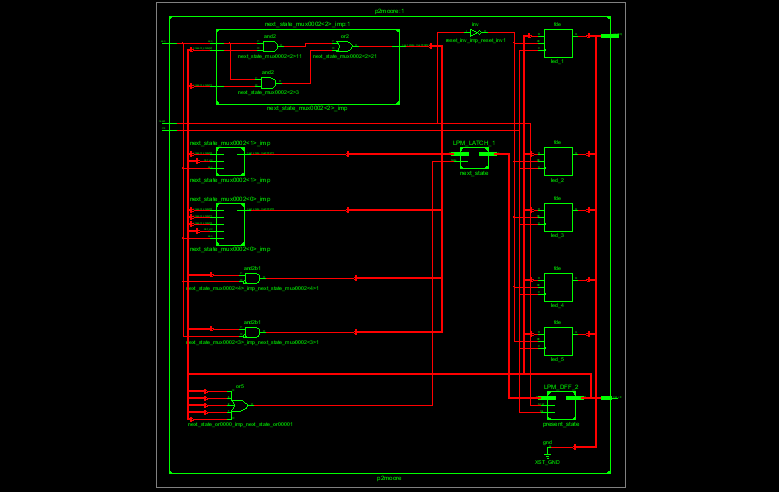
\includegraphics[scale=0.8, center]{images/screenshot21}
	\caption{Screenshot for problem statement 2}
	\end{figure}
	\pagebreak
	\begin{figure}[h!]
	\centering
	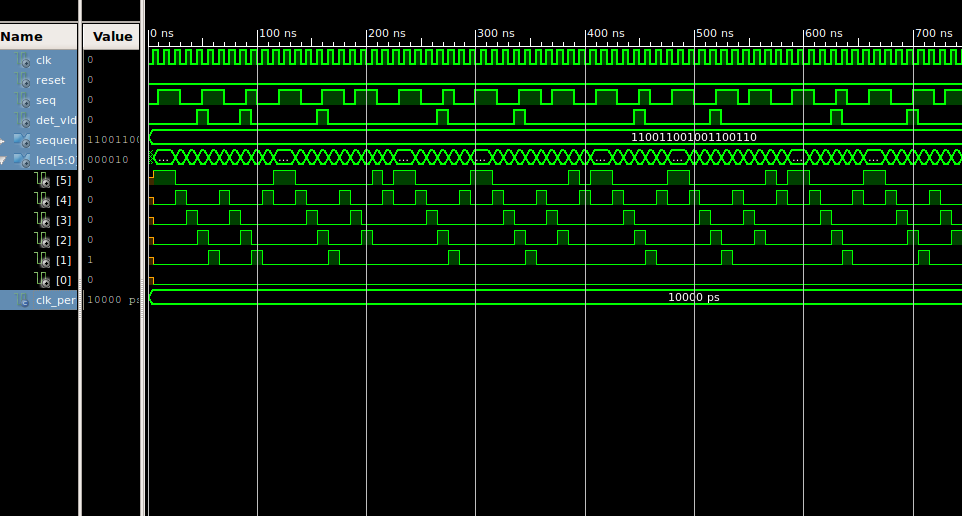
\includegraphics[scale=0.8, center]{images/screenshot22}
	\caption{Screenshot for problem statement 2}
	\end{figure}
	\pagebreak
	\begin{figure}[h!]
	\centering
	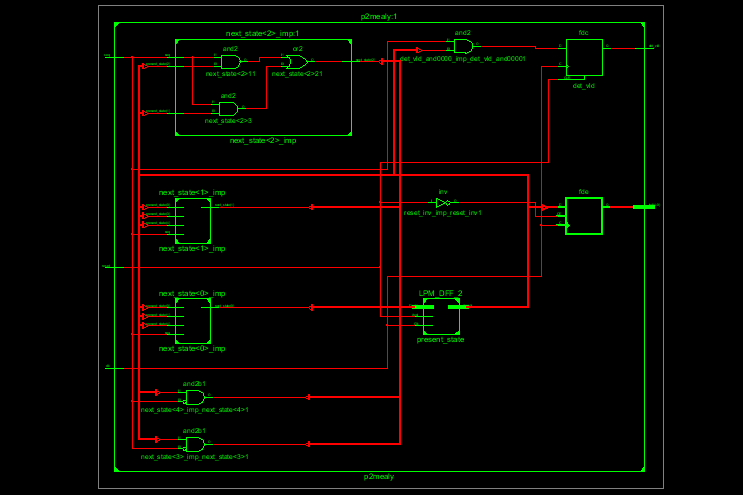
\includegraphics[scale=0.8, center]{images/screenshot23}
	\caption{Screenshot for problem statement 2}
	\end{figure}
	\pagebreak
	\begin{figure}[h!]
	\centering
	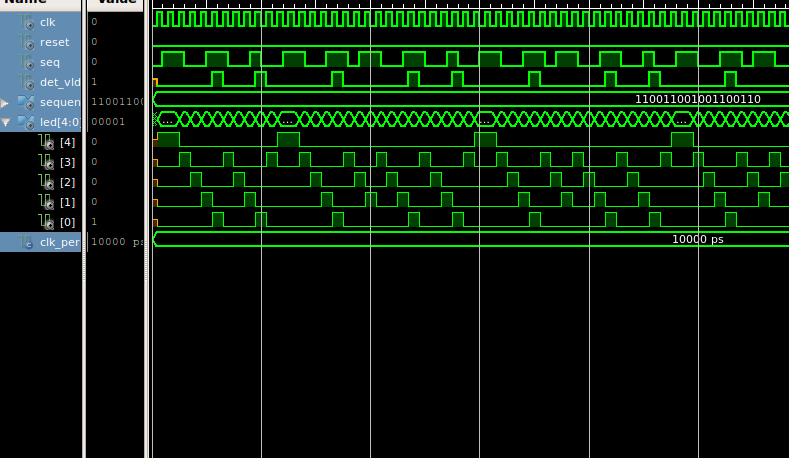
\includegraphics[scale=0.6, center]{images/screenshot24}
	\caption{Screenshot for problem statement 2}
	\end{figure}
	\pagebreak
	\begin{figure}[h!]
	\centering
	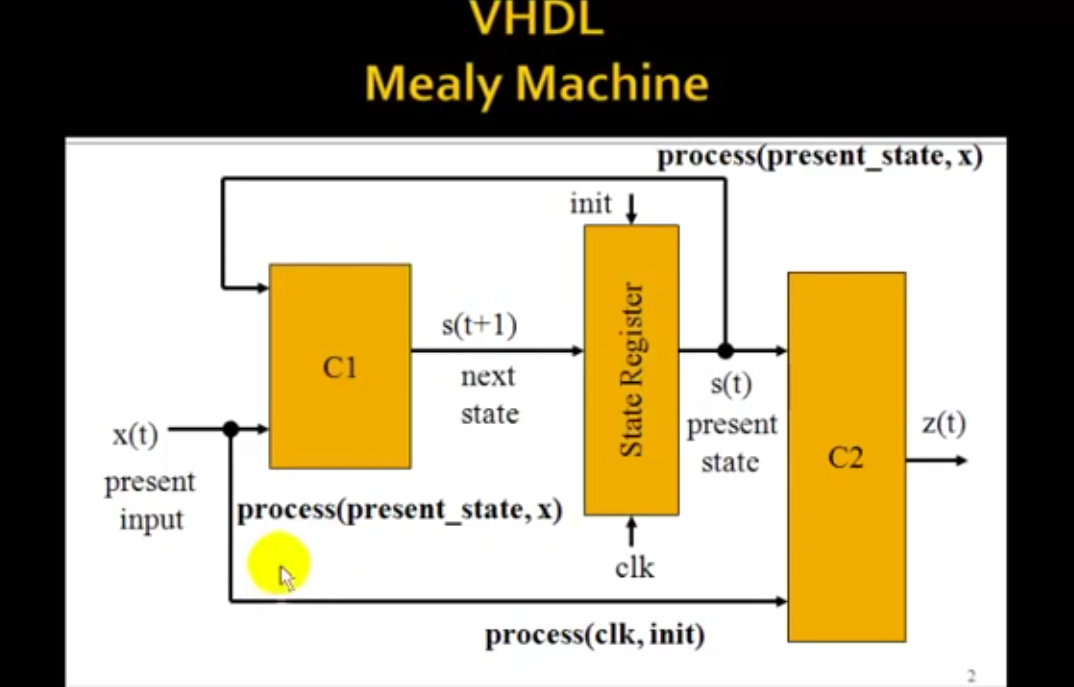
\includegraphics[scale=0.6, center]{images/screenshot25}
	\caption{Screenshot for problem statement 2}
	\end{figure}
	\pagebreak
	\begin{figure}[h!]
	\centering
	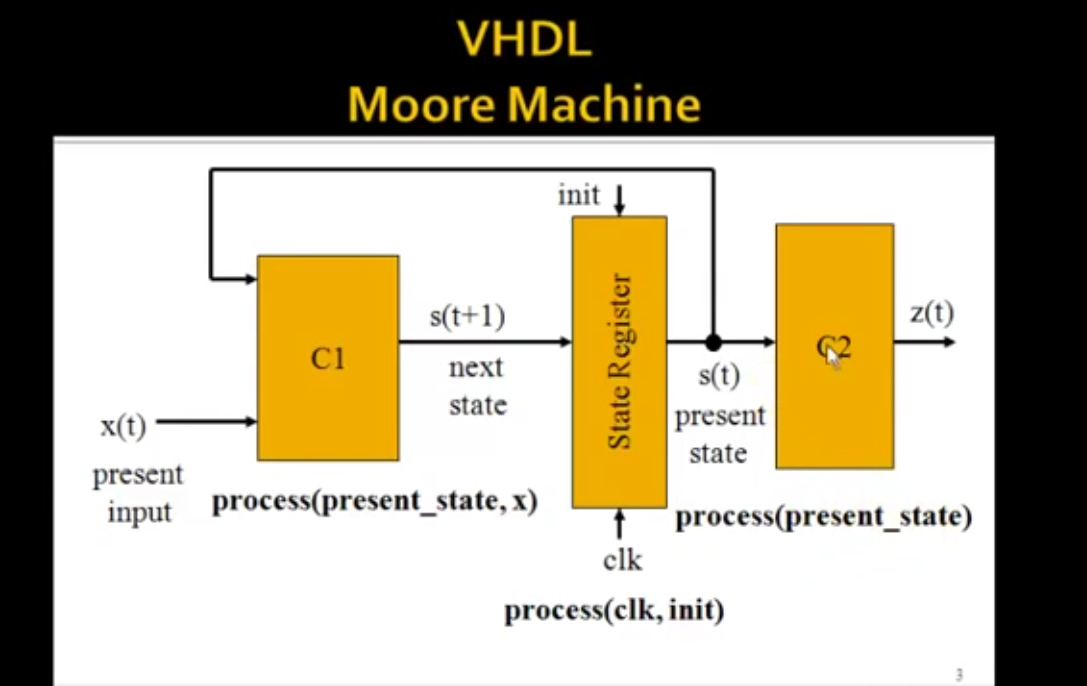
\includegraphics[scale=0.6, center]{images/screenshot26}
	\caption{Screenshot for problem statement 2}
	\end{figure}
	\pagebreak
%\section{Problem Statement 3}
%\textbf{Part - 1 -}\\
%Write shell script to emulate behaviour of bash, but also record every command put up on terminal on a logger.txt file along with time stamp. Your command prompt should look like normal bash command prompt. \\
%	\subsection{Assumptions}
%	The output is to be processed in the exact manner as shown in the image\\
%	\begin{figure}[h!]
%	\centering
%%	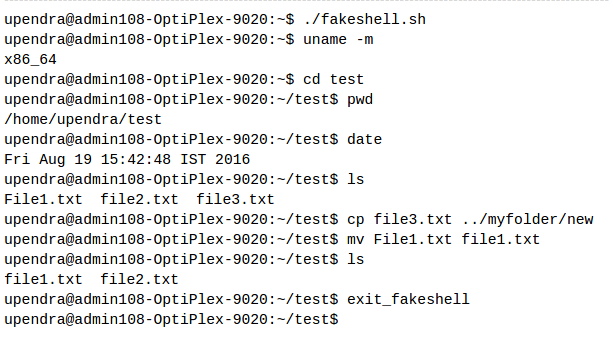
\includegraphics[scale=0.7]{images/Selection_004}	
%	\end{figure}
%	\pagebreak
%	\subsection{Structure Chart}
%	\begin{figure}[h!]
%	\centering
%	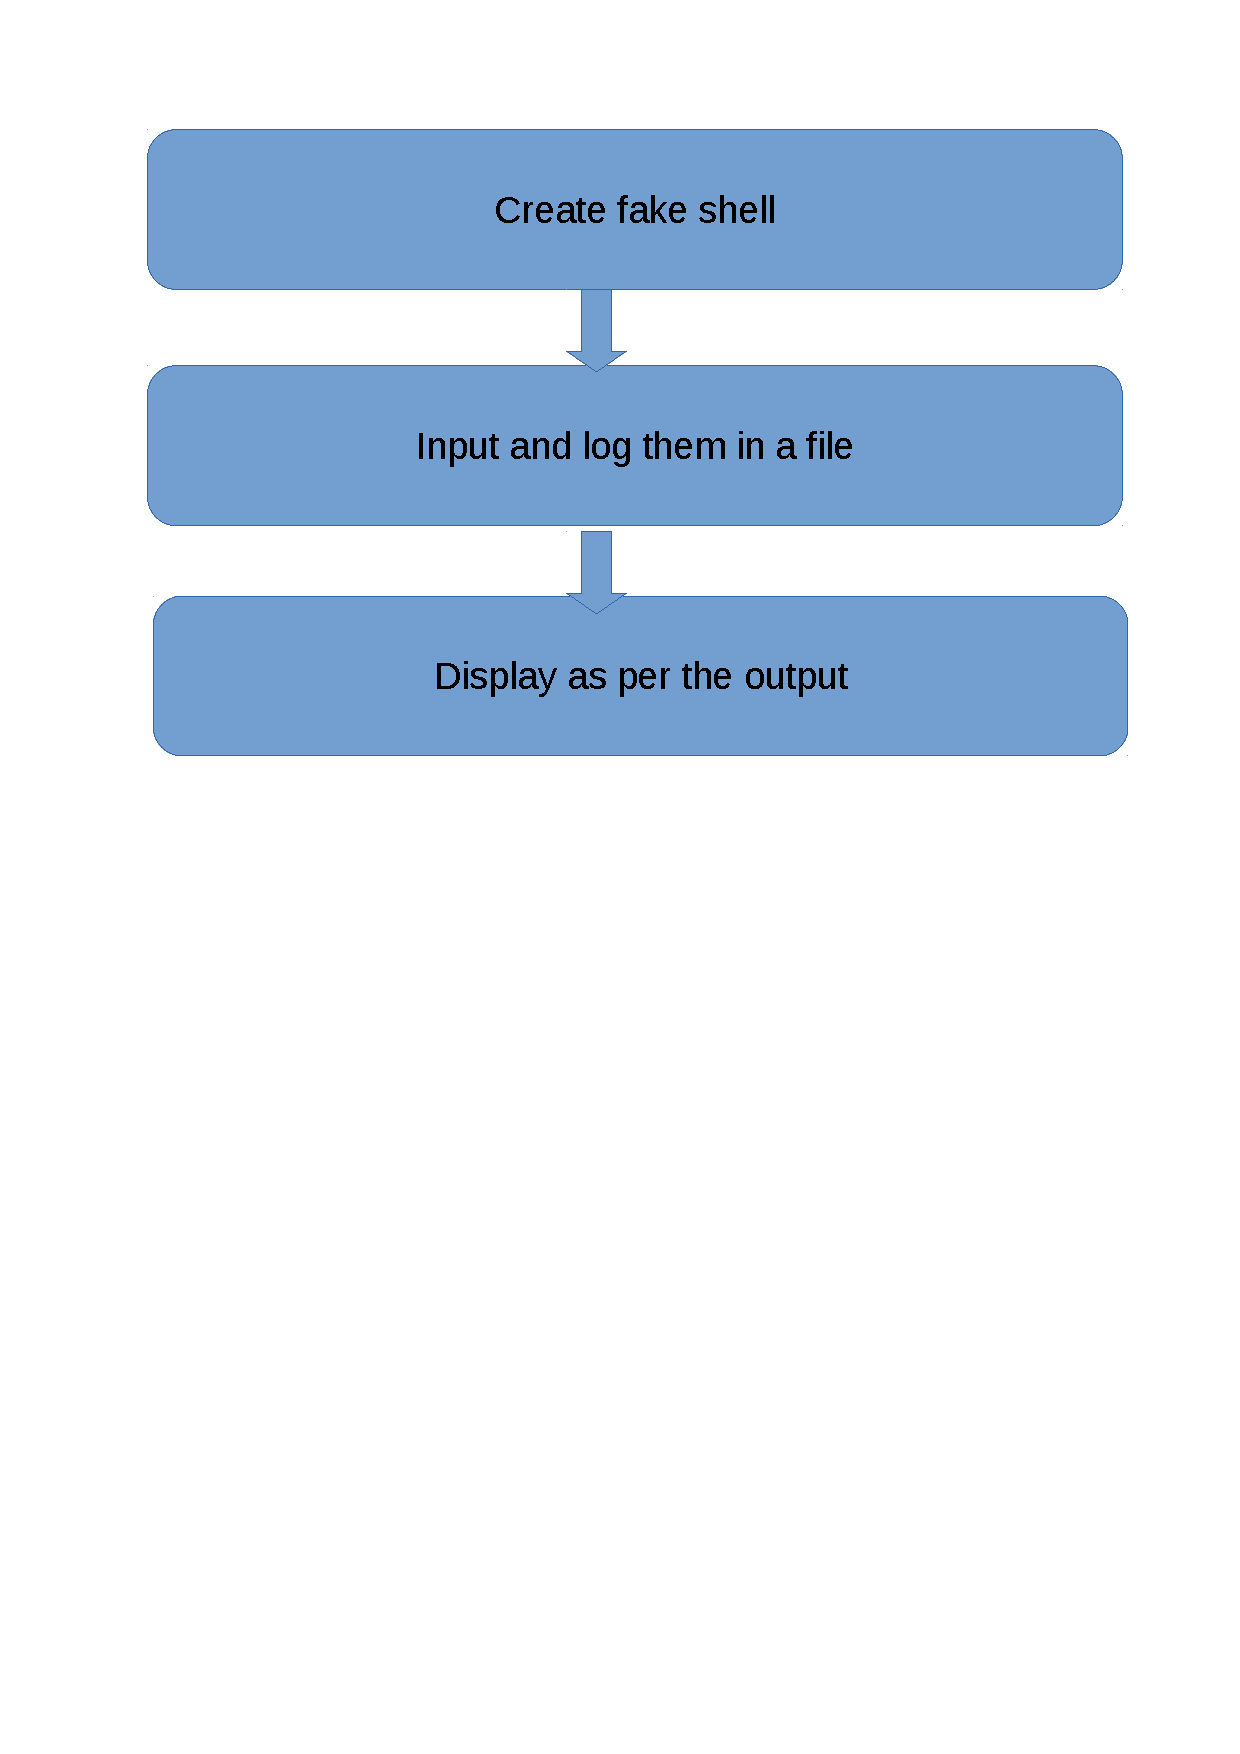
\includegraphics[scale=0.7]{images/shots33}
%	\caption{Structure chart for problem 3}	
%	\end{figure}
%	\pagebreak
%	%\fi
%	\pagebreak
\section{Epilogue}
The execution of the first problem involved writing of a vhdl module with a testbench.The module had two buses that were to be compared with each other.
The execution of the second statement had been done in two ways - Moore machine and mealy machine. \\ 
Mealy machine : 
A Mealy Machine is an FSM whose output depends on the present state as well as the present input. The mealy machine has 5 finite states and the corresponding implementation has been shown here.
Moore machine :
Moore machine is an FSM whose outputs depend on only the present state. Moore machine has 6 finite states and the difference in implementation can be observed in the code. 
\bibliography{biblio}
\bibliographystyle{ieeetr}
\nocite{*}
\end{document}